%!TEX root = ../template.tex
%%%%%%%%%%%%%%%%%%%%%%%%%%%%%%%%%%%%%%%%%%%%%%%%%%%%%%%%%%%%%%%%%%%%
%% chapter2.tex
%% NOVA thesis document file
%%
%% Chapter with the template manual
%%%%%%%%%%%%%%%%%%%%%%%%%%%%%%%%%%%%%%%%%%%%%%%%%%%%%%%%%%%%%%%%%%%%

\typeout{NT FILE chapter2.tex}%

\chapter{Work plan}
\label{cha:work_plan}


\section{Characterization of the solution}
\label{sec:characterization_of_the_solution}

 The IOPT-Tools environment provides robust support for modeling, verifying, and generating code for individual controller sub-models using Input-Output Place-Transition (IOPT) Petri nets \cite{iopttools, barros2004, RefiningIOPT}. However, a notable challenge arises in distributed control systems, particularly those adhering to the Globally Asynchronous, Locally Synchronous (GALS) paradigm, where decomposed sub-models require inter-communication \cite{galsactd, Barrosadd}. As identified in Section~\ref{subsec:communication_gap}, the existing automatic code generation primarily focuses on the internal logic of each sub-model, necessitating manual implementation of the communication links between them. This dissertation directly addresses this gap by proposing an automated code generation tool. The core objective is to develop a mechanism that analyzes decomposed IOPT sub-models and automatically generates the necessary communication infrastructure code. This tool is envisioned to streamline the development of distributed control systems by automating the creation of efficient and reliable data exchange pathways. The anticipated output is a tool capable of producing C code for microcontroller-based systems and VHDL for Field-Programmable Gate Array (FPGA) implementations \cite{barros2004, vhld}. This generated communication code will integrate with the controller logic produced by IOPT-Tools, thereby reducing development effort, minimizing manual coding errors, and enhancing the overall utility of the IOPT-Tools framework for complex distributed applications.

A draft propossed is the following:

Implement code C or VHDL in the Receviever/ Transmitor module of each controller ~\ref{fig:representation}
\begin{figure}[htbp]
  \centering
  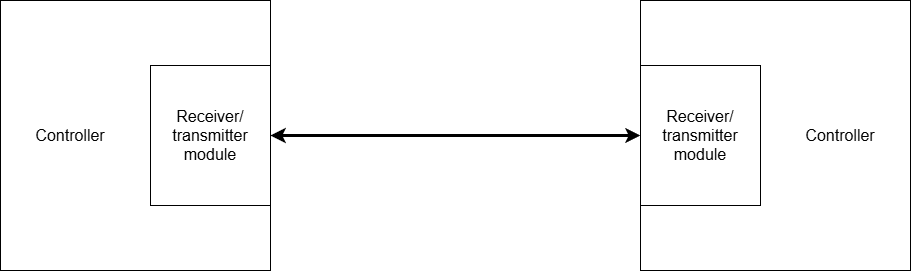
\includegraphics[width=0.6\textwidth]{Chapters/Figures/Diagrama.png}
  \caption{Solution representation.}
  \label{fig:representation}
\end{figure}


The proposed implementation facilitates code generation within the IOPT tool suite through an enhanced graphical user interface. As depicted in Figure~\ref{fig:butao}, the solution introduces a new button that initiates a guided configuration workflow. Upon initiation, a window is presented (Figure~\ref{fig:11}), prompting the user to select the requisite input files in the .pnml format. Following file selection, the user proceeds to define the system's communication channels and assign the desired communication technology for each, with options including I2C, SPI, UART, and FIFO with Handshake Figure~\ref{fig:12}. The final window in this workflow, illustrated in Figure~\ref{fig:improgress}, allows for the selection of protocol-specific characteristics and the designation of the target output language, such as C or VHDL.


\begin{figure}[htbp]
  \centering
  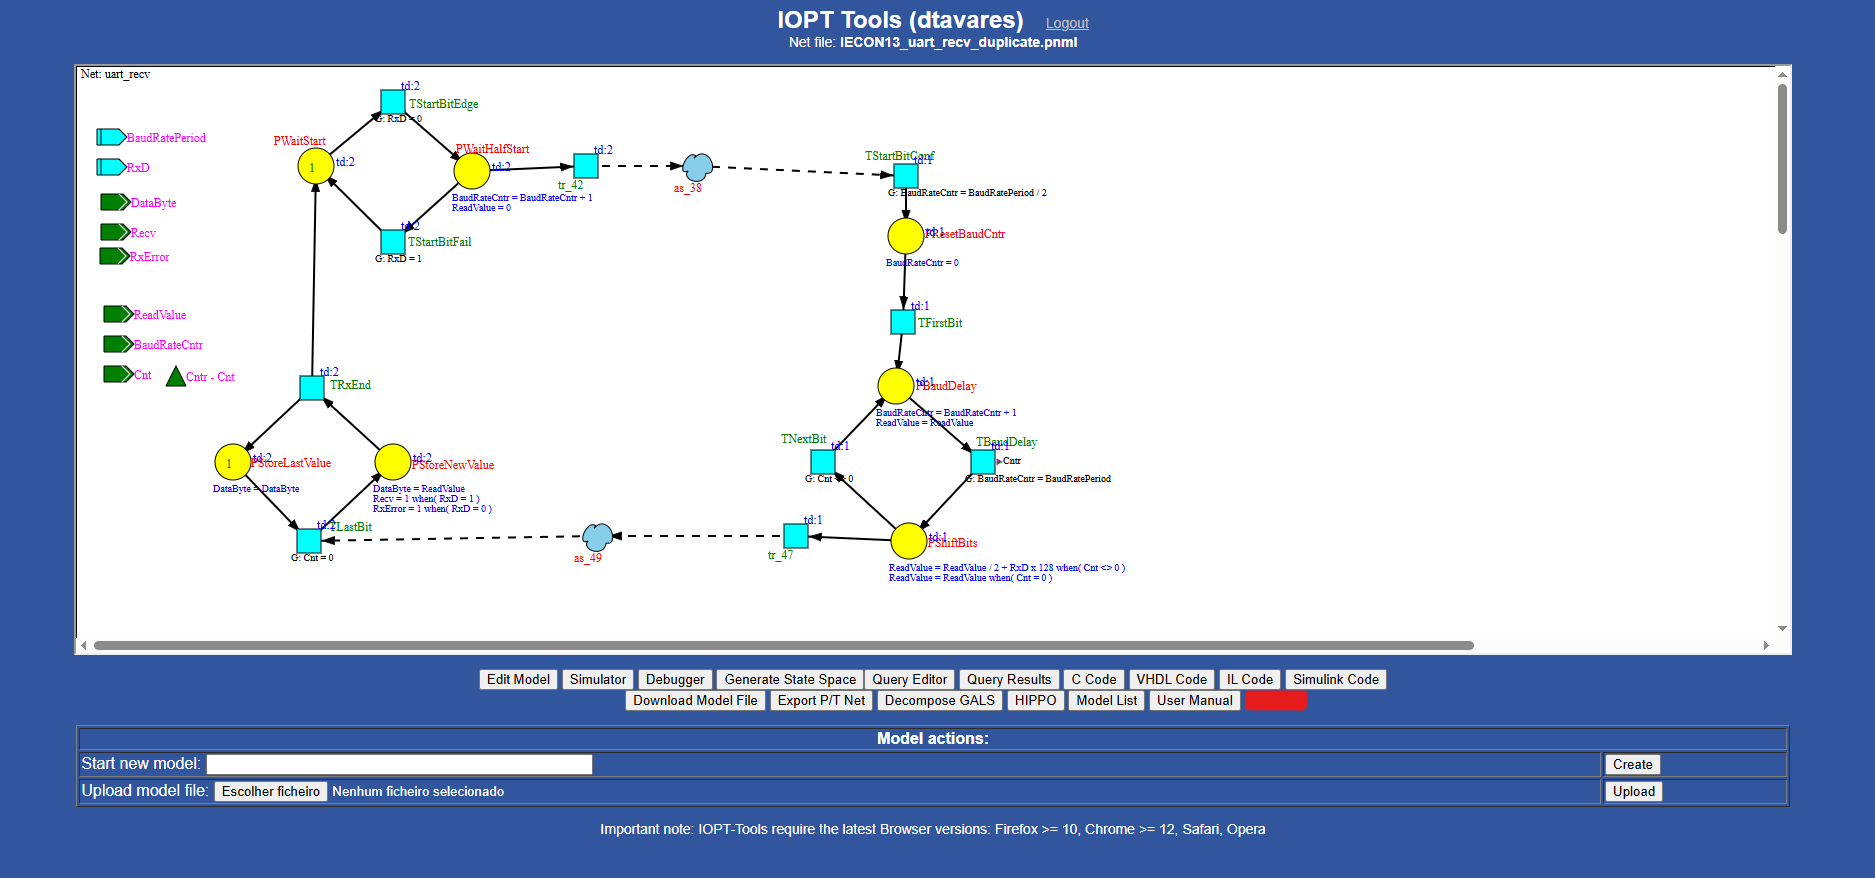
\includegraphics[width=0.6\textwidth]{Chapters/Figures/butao.png}
  \caption{Solution representation.}
  \label{fig:butao}
\end{figure}
\begin{figure}[htbp]
  \centering
  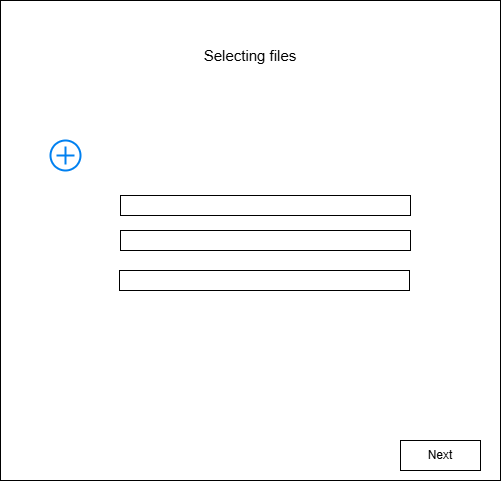
\includegraphics[width=0.6\textwidth]{Chapters/Figures/11.png}
  \caption{Solution representation2.}
  \label{fig:11}
\end{figure}
\begin{figure}[htbp]
  \centering
  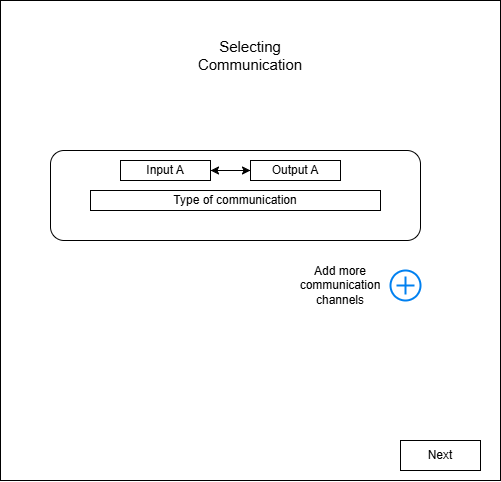
\includegraphics[width=0.6\textwidth]{Chapters/Figures/12.png}
  \caption{Solution representation3.}
  \label{fig:12}
\end{figure}
 
 
 
 
 
 
\section{Gant Diagram }
\label{sec:gant_diagram}

Gant diagram

\section{Task building}
\label{sec:task_building}

enumerar as tarefas que irei fazer
